\documentclass{article} % For LaTeX2e
\usepackage{nips12submit_e,times}
\usepackage{graphicx}
\usepackage{hyperref}
\usepackage{wrapfig}

%\documentstyle[nips12submit_09,times,art10]{article} % For LaTeX 2.09


\title{Facebook's Mapping the Internet Kaggle Competition \\
{\small CSE599 Machine Learning for Big Data Term Project Report}}


\author{Nicole Deflaux \\
University of Washington Non-Matriculated Student, ID 1210660 \\
\texttt{nicole.deflaux@gmail.com}
}

\newcommand{\fix}{\marginpar{FIX}}
\newcommand{\new}{\marginpar{NEW}}

%\nipsfinalcopy % Uncomment for camera-ready version

\begin{document}

\maketitle

\begin{abstract}
  This project applied online machine learning techniques appropriate for
  Big Data problems to the task of interdomain routing.
\end{abstract}

% \tableofcontents

\section{Project Idea}
``The Task: you will be given a path which, at one point in the training time
period, was an optimal path from node A to B. The question is then to make a
probabilistic prediction, for each of the 5 test graphs'' which are
unobserved, ``whether the given path is STILL an optimal path.  This is a
much more difficult task than link prediction alone. The global structure of
the graph may affect many optimal routes, paths can have varying lengths
(and thus varying a priori probabilities of being optimal), and there may be
multiple optimal routes for a given source and destination.''~\cite{kaggle}

\subsection{Data}

\begin{wrapfigure}{r}{0.25\textwidth}
  \begin{center}
    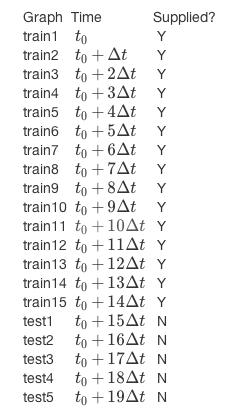
\includegraphics[scale=.5]{trainAndTestGraphs.png}
  \end{center}
\end{wrapfigure}

The domain of the data in this problem are the connections between
autonomous systems~\cite{asn} in the Internet.  More specifically, the nodes
in the graph correspond to gateway routers for independent networks, and the
directed edges between them encode the network peering relationships with
edge weight indicating the cost type of transit over those links.

The training dataset consists of 15 graphs with anywhere from 46,603 to 49,520 directed edges each (so on the
order of $\approx$750,000 edges total).  Each graph was collected at sequential time
points indicating operational direct connections and their cost types in the
network known at that point in time.  The format of each edge in the
training graph is \texttt{tail router AS Name | head router AS
  Name | cost type for use of the link} where the cost type is either 0 for ``free'' or 1
indicating that a fee is to be paid.  The number of unique node names in the
training dataset is 372,037 but part of the competition is to figure out
which of those "messy" names are duplicates.  A training edge may look like:

\texttt{{\small GOOGLE-CORPNET Google Ireland Limited | FACEBOOK-CORP - Facebook Inc | 1}}

The test dataset consists of 10,000 single or multi-edge paths for the (unobserved)
graphs at the next five time intervals.  A test path may look like:

\texttt{{\small REDWIRE - VoloNet Technologies, Inc | NCN-AS FOP Sergey Sergeevich | DKB | JMC-AS - JPMorgan Chase \& Co. | PIERCE-COUNTY - Pierce County}}

\subsection{Approach and Challenges}

Although this competition could have been performed using batch machine
learning, for the purposes of this project the problem was reformulated as
one for online machine learning.  The edges in each training graph were
randomly permuted and then fed incrementally to the learning algorithm, with
all the edges of graph 1 streamed prior to those of graph 2, etc...

Note that to meet the goals of this competition, two models were needed: (1)
a classification model for edge existence and (2) a classification model for
edge cost type.  Both were learned incrementally as the edge data streamed in.

\textbf{Challenges}
\begin{itemize}
\item changing dimensionality of feature space: edges will come and go with time
\item temporality: edges will change costs with time
\item incomplete data: edges may be absent from the data but still exist
\item messy data: node names are mangled in the data and de-duping is needed
\end{itemize}

\section{Implementation}

The code for this implementation is hosted on github
\url{https://github.com/deflaux/rework/tree/master/competitions/facebook2}
and consists of Java, Python, and R code.

% \begin{verbatim}
% ~/rework/competitions/facebook2>find . -name *.java | xargs cat | wc -l
%     2352
% ~/rework/competitions/facebook2>find . -name *.py | xargs cat | wc -l
%      571
% ~/rework/competitions/facebook2>find . -name *.R | xargs cat | wc -l
%       80
% ~/rework/competitions/facebook2>find src/main/ -name *.java | xargs cat | wc -l
%     1130
% \end{verbatim}

\subsection{Data Cleaning}

Preprocessing was performed to compute a mapping of ``messy'' names to
opaque keys.  An example is showing in Figure~\ref{fig:mess}.  The software was able to reduce the number of unique node
names in the training and test data from 384,644 to 22,580.  Additional
results from the data cleaning process can be seen in Table~\ref{tab:clean}.

\begin{table}
\begin{tabular}{rrl} 
\textbf{Raw Data} & \textbf{Cleaned Data} & \\
372,042 & 22,568 & unique node names in training data \\ 
23,991 & 9,454 & unique node names in test paths\\
12,602 & 12 & unique node names in test paths but not in training data\\
544,428 & 67,612 & unique edges in training data \\
34,492 & 15,491 & unique edges in test paths \\
31,208 & 236 & unique edges in test paths but not in training data \\
87,468 & 13,937 & unique free cost type edges in training data \\
458,171 & 55,439 & unique paid cost type edges in training data \\
1,211 & 1,764 & unique edges that changed cost type in training data \\
22 & 9,672 & number of test paths for which we have training data for all edges
in the path \\
NA & 215 & unique nodes names only used in a single edge \\
\end{tabular}
\caption{Data Cleaning Results}
\label{tab:clean}
\end{table}

\begin{figure}
\texttt{abccefkooopr abcefkoo cin | 38 | ['FACEBOOK-CORP Inc - Facebook Inc', 'Facebook FACEBOOK-CORP - Facebook Inc', 'O-BEFKORACOPC - Facebook Inc', \textbf{...} 'FACEBOOK-CORP - boackFeo Inc', 'FACEBOOK-CORP Facebook - Facebook Inc', '- Facebook Inc', 'FACEBOOK-CORP - Facebook Facebook Inc', 'FACEBOOK-CORP - Facebook ncI', 'FACEBOOK-CORP - Facebook Inc Inc', 'FACEBOOK-CORP FACEBOOK-CORP - Facebook Inc']}
\caption{A mapping of a single key to 38 ``messy'' names}
\label{fig:mess}
\end{figure}

% \begin{tabular}{rl} 
% 22,568 &  unique node names in training data \\ 
% 9,454 &  unique node names in test paths\\
% 12 &  unique node names in test paths but not in training data\\
% 67,612 &  unique edges in training data \\
% 15,491 &  unique edges in test paths \\
% 236 &  unique edges in test paths but not in training data \\
% 13,937 &  unique free cost type edges in training data \\
% 55,439 &  unique paid cost type edges in training data \\
% 1,764 &  unique edges that changed cost type in training data \\
% 9,672 & number of test paths for which we have training data for all edges
% in the path \\
% 215 & unique nodes names only used in a single edge \\
% \end{tabular}

% V1 O(n) Software was written to normalize and deduplicate the ``messy'' node names
% found in the input data.  Techniques such as tf-idf were used to determine
% which term(s) to remove from a multi-word node name to see if it
% corresponded to a shorter word name. 

% union find

% V2 O(n^2)

\subsection{Features}

\textbf{Modeling Connections} A feature is created for each $tail
\rightarrow head$ pair and then hashed~\cite{hash} into a constrained dimensional
space since, for this task reformulated as online learning, the true
dimensionality of our input space will change.

\textbf{Modeling Connectedness} Features are created for the $head$ and
$tail$ of each edge and then hashed~\cite{hash} into the same constrained dimensional
space.  There are some nodes in the data which are very high degree and
likely to be robust in terms of existence.  This feature attempts to
approximate the degree of each node per the data streamed in.

\textbf{Modeling Temporality} Features are created from a sliding window of
past information from prior epochs about existence and cost of the edge.
Bloom filters are used to compactly store this high dimensional historical
data.

Note that time is a very important factor in this model.  In this
reformulated version of the problem, information about
the network is continually streaming in.  The notion of epoch is used to
indicate a interval of time during which we would expect to receive the
state from \emph{most} nodes in the graph.

This notion of epoch maps onto the training data such that all edges from
\texttt{train1.txt} regardless of their order are considered to be in epoch
1, all edges from \texttt{train2.txt} regardless of their order are
considered to be in epoch 2, ... all edges from \texttt{train15.txt}
regardless of their order are considered to be in epoch 15.  Therefore
when we train upon an edge at time $t$ the function $epoch(t)$ is defined as
$epoch(t) \in {1, ..., 15}$ corresponding to the training graph from which
the edge came.\footnote{In a more realistic situation, the duration of an
  epoch might be 5 minutes, or 30 minutes, or an hour; when we train upon an
  edge at time $t$ the function $epoch(t)$ is defined as $epoch(t) \in N$
  monotonically increasing as each epoch duration elapses.}

\subsection{Models}

\subsubsection{Edge Existence Model}

Let $u$ and $v$ be two nodes in the graph at time $t$.  Then we have the
binary label $y_{exists\{u \rightarrow v\}}^{(t)} \in \{0,1\}$ where $1$
means that an edge exists directly between $u$ and $v$, $0$ that the edge
does not exist.  Note that in our training data we only have labels where
$y_{exists\{u \rightarrow v\}}^{(t)} = 1$.

% Edges missing from the training data are assumed $y_{exists\{u \rightarrow
%   v\}}^{(t)} = 0$.  

We have the feature vector $x_{exists\{u \rightarrow v\}}^{(t)} \in R^{d+h}$
which is a column vector of length $d+h$ where
\begin{itemize}
\item $d$ is the dimension of the space into which we have hashed our edge,
  tail, and head names
\item $h$ is the size of the sliding window of historical data
\end{itemize}

For a particular edge $u \rightarrow v$ and the current epoch, the feature
vector will hold the following values:
\begin{itemize}
\item The first $d$ values in $x$ are sparse.  The only entries that will
  have values are the hashed entries for the edge, tail, and head names of
  edge $u \rightarrow v$.
\item The next $h$ values in $x$ are binary indicators of the existence for
  edge $u \rightarrow v$ at $epoch(t)-1, epoch(t)-2, ..., epoch(t)-h$.
\end{itemize}

\subsubsection{Edge Cost Type Model}
Let $u$ and $v$ be two nodes in the graph at time $t$.  Then we have the
binary label $y_{cost\{u \rightarrow v\}}^{(t)} \in \{0,1\}$ where $0$ means
that a fee must be paid for traffic traversing the edge directly between $u$
and $v$ and $1$ means that there is no fee.\footnote{This is the reverse of
  the costs in the raw data.}

We have the features vector similar to the existence model $x_{cost\{u
  \rightarrow v\}}^{(t)} \in R^{d+h}$ which is a column vector of length
$d+h$ where
\begin{itemize}
\item $d$ is the dimension of the space into which we have hashed our edge,
  tail, and head names
\item $h$ is the size of the sliding window of historical data
\end{itemize}

For a particular edge $u \rightarrow v$ and the current epoch, the feature
vector will hold the following values:
\begin{itemize}
\item The first $d$ values in $x$ are sparse.  The only entries that will
  have values are the hashed entries for the edge, tail, and head names of
  edge $u \rightarrow v$.
\item The next $h$ values in $x$ are binary indicators of cost type free for
  edge $u \rightarrow v$ at  $epoch(t)-1, epoch(t)-2, ..., epoch(t)-h$.  Note that when building
  this portion of the feature vector, if the edge did not exist during
  $epoch(t)-j$ where $j < h$ we backfill the with cost value from the most
  recently observed prior epoch.
\end{itemize}

\subsection{Learning Algorithm}

Stochastic gradient descent~\cite{rand}\cite{online} was used to train both models.

\begin{displaymath}
w_i^{(t+1)} = w_i^{(t)} + \eta \{- \lambda w_i^{(t)} + x_i^{(t)} [ y^t -  Prob(Y=1|x^{(t)},w^{(t)})] \}
\end{displaymath}

where
\begin{displaymath}
Prob(Y=1|x^{(t)},w^{(t)}) = \frac{exp(\sum_{k=1}^{d+h} w_kx_k)}{1+exp(\sum_{k=1}^{d+h} w_kx_k)}
\end{displaymath}

Note that during each training step, we are also recording history.  When we
train upon edge $u \rightarrow v$ at time $t$ the edge is added to the
existence bloom filter associated with $epoch(t)$.  If it is of the free
cost type, it is also added to the cost bloom filter associated with
$epoch(t)$.

\subsection{Optimality Prediction Process}
\label{sec-pred}

Prediction for this Kaggle competition consists of multiple steps.  For each
of the unobserved graphs for epochs 16 through 20:

\begin{enumerate}
\item First predict the graph for epoch 16.  To do this, for each possible edge in the graph:
  \begin{enumerate}
  \item predict whether the edge in the graph exists during epoch 16
  \item if the prediction is true, then predict its cost type
  \end{enumerate}
\item Then determine the optimality of the test paths.  To do this, for each path in the test paths:
  \begin{enumerate}
  \item compute the cost of the test path in our predicted graph for epoch 16
  \item use Dijkstra's algorithm to compute cost of the shortest path in the
    predicted graph between the tail and the head of the test path
  \item if the costs are equal, the path is still ``optimal'' in epoch 16
  \end{enumerate}
\end{enumerate}

Repeat this for epochs 17 through 20.

\section{Current Results}

Some amount of model parameter tuning was performed and the chosen
parameters are shown in Table~\ref{tab:param}.

\begin{table}
\begin{tabular}{rrl} 
\textbf{Existence Model} & \textbf{Cost Model} & \textbf{Parameter} \\
10 & 10 & $h$ history sliding window size\\
65,536 & 65,536 & $d$ dimensionality of hashed text feature\\
0.05 & 0.05 & $\eta$ step size of stochastic gradient descent\\
0.1 & 0.001 & $\lambda$ regularization for stochastic gradient descent\\
\end{tabular}
\caption{Model parameters used for the current results}
\label{tab:param}
\end{table}

\subsection{Training Performance}

For both models, the training data was skewed. For the existence model,
\emph{all data} was positive.  For the cost model, only 17\% of edges were of
the free cost type.  Training performance improved over time in general, but
not always, as shown in Figure~\ref{fig:loss} and Figure~\ref{fig:avgloss}.

\begin{figure}
  \begin{center}
    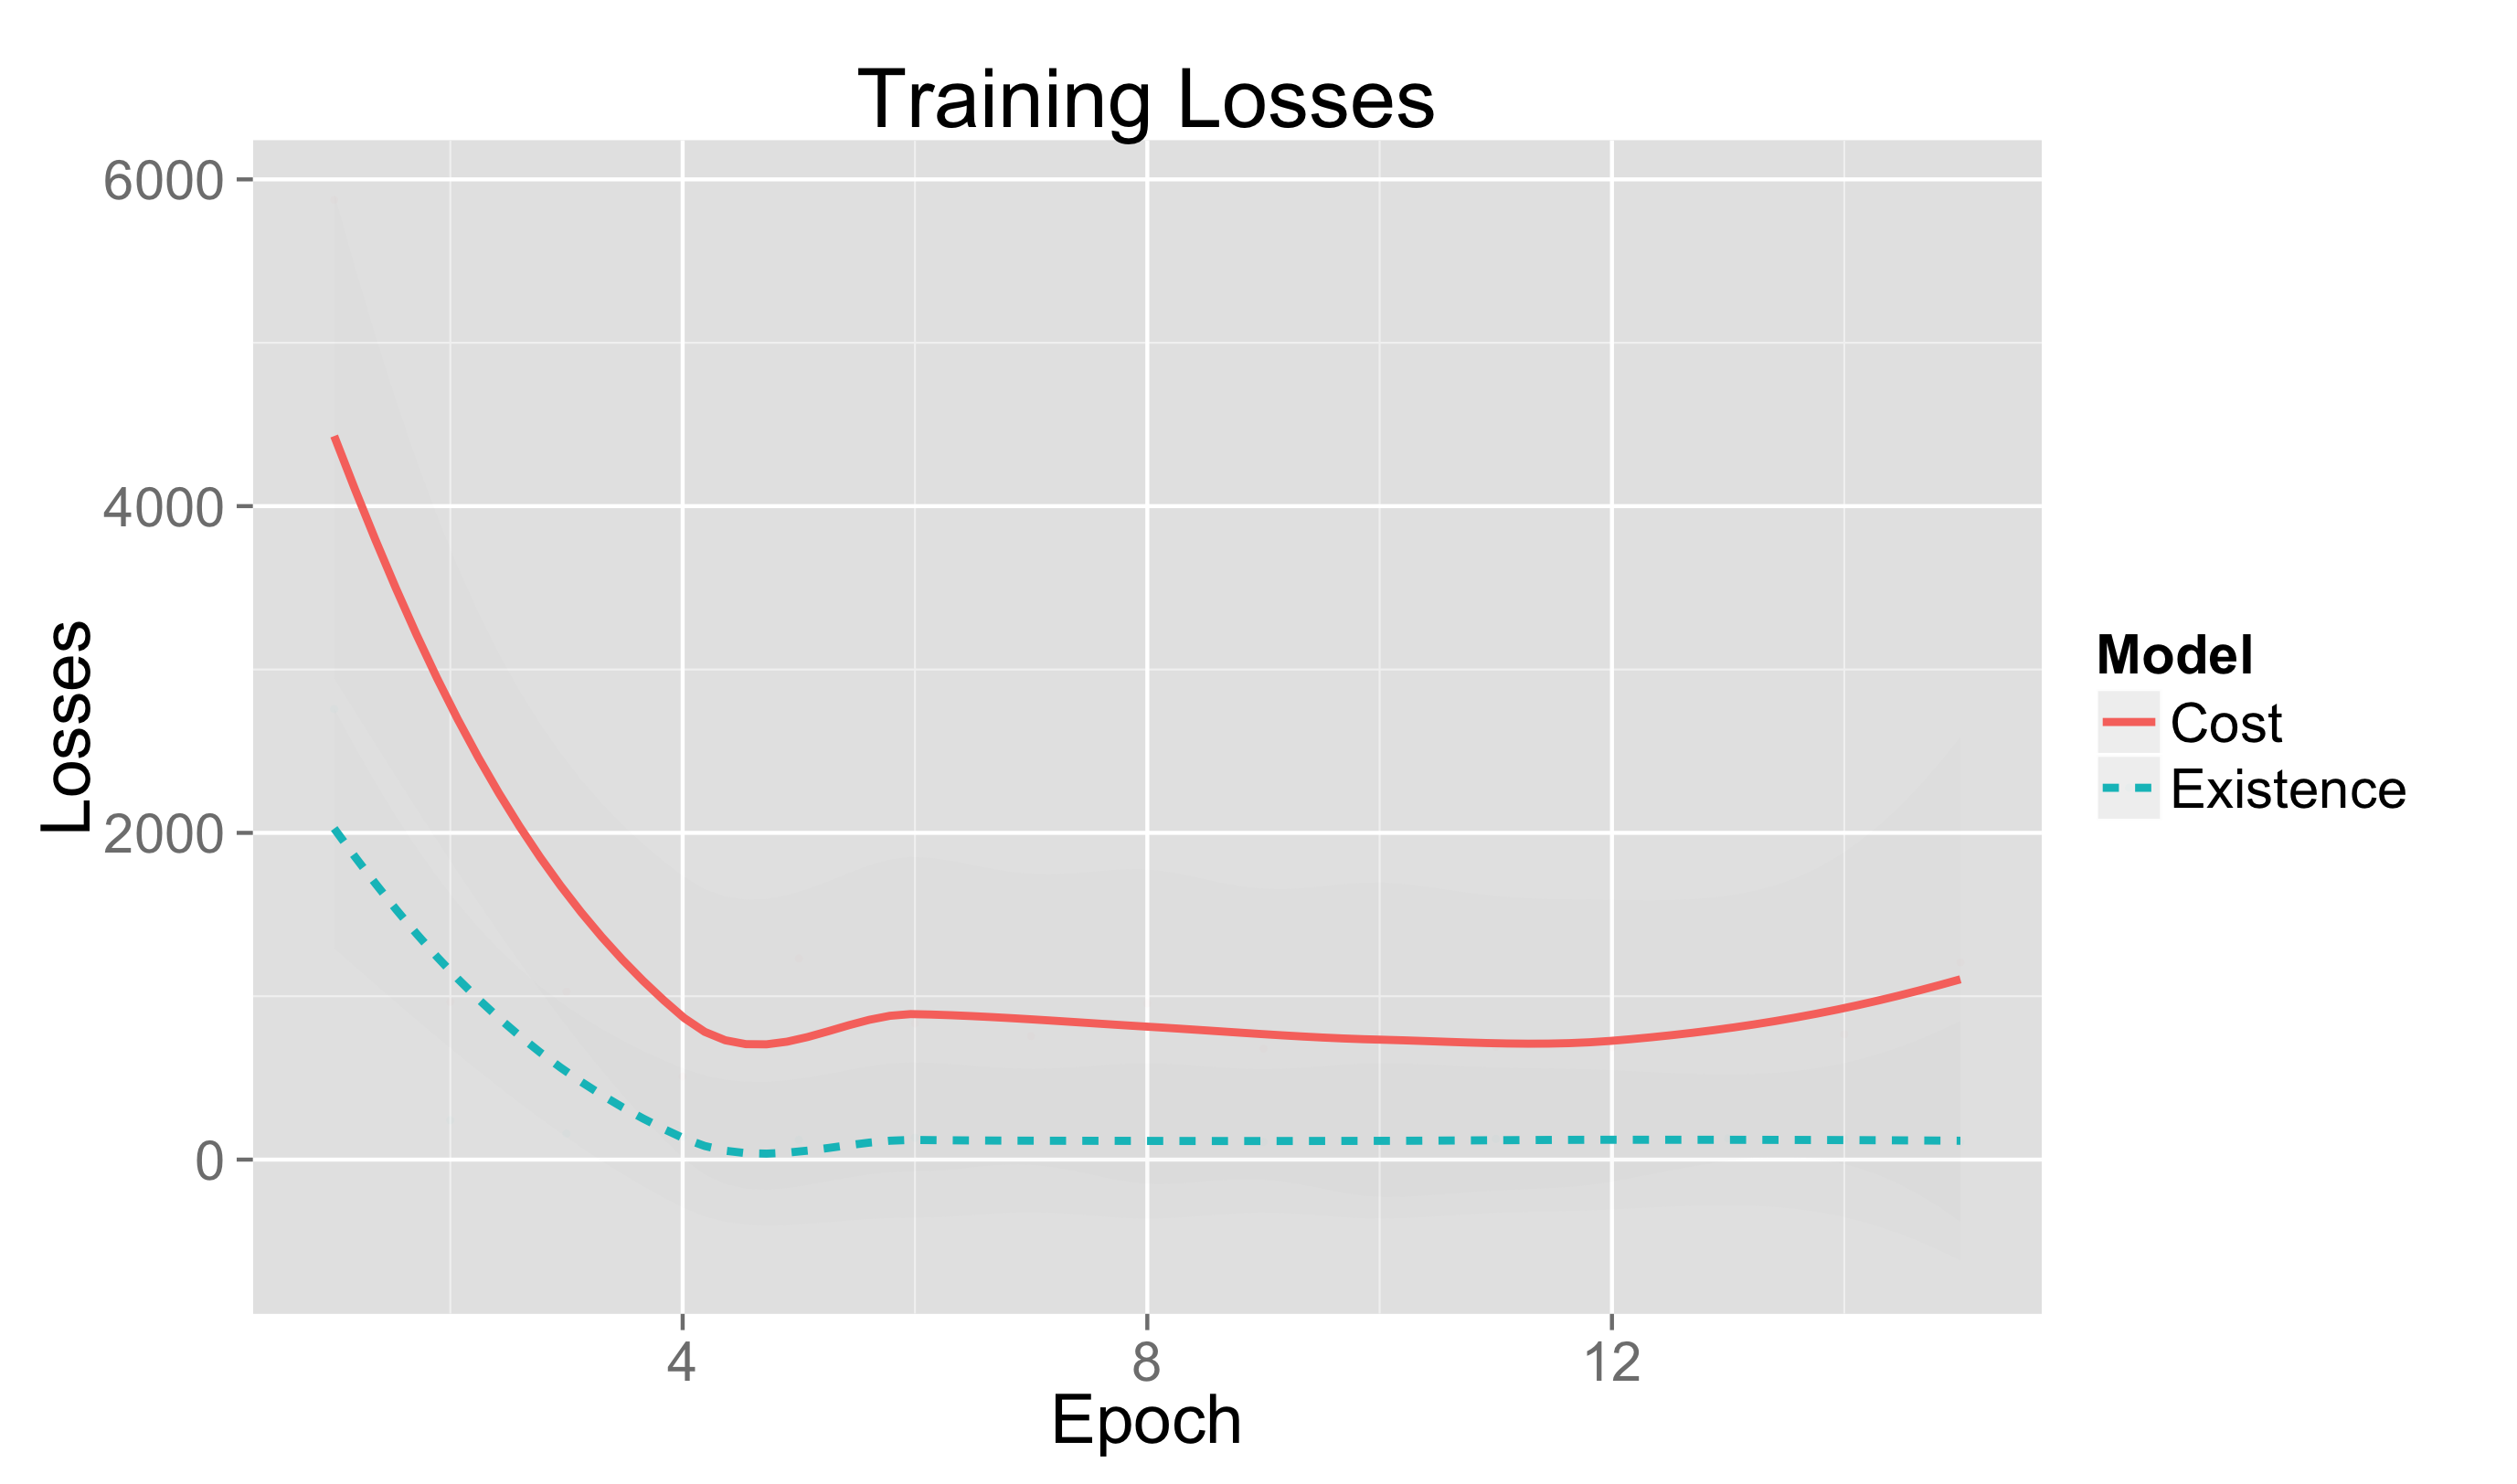
\includegraphics[scale=.1]{trainingLosses.png}
  \end{center}
  \caption{Training losses per epoch}
  \label{fig:loss}
\end{figure}

\begin{figure}
  \begin{center}
    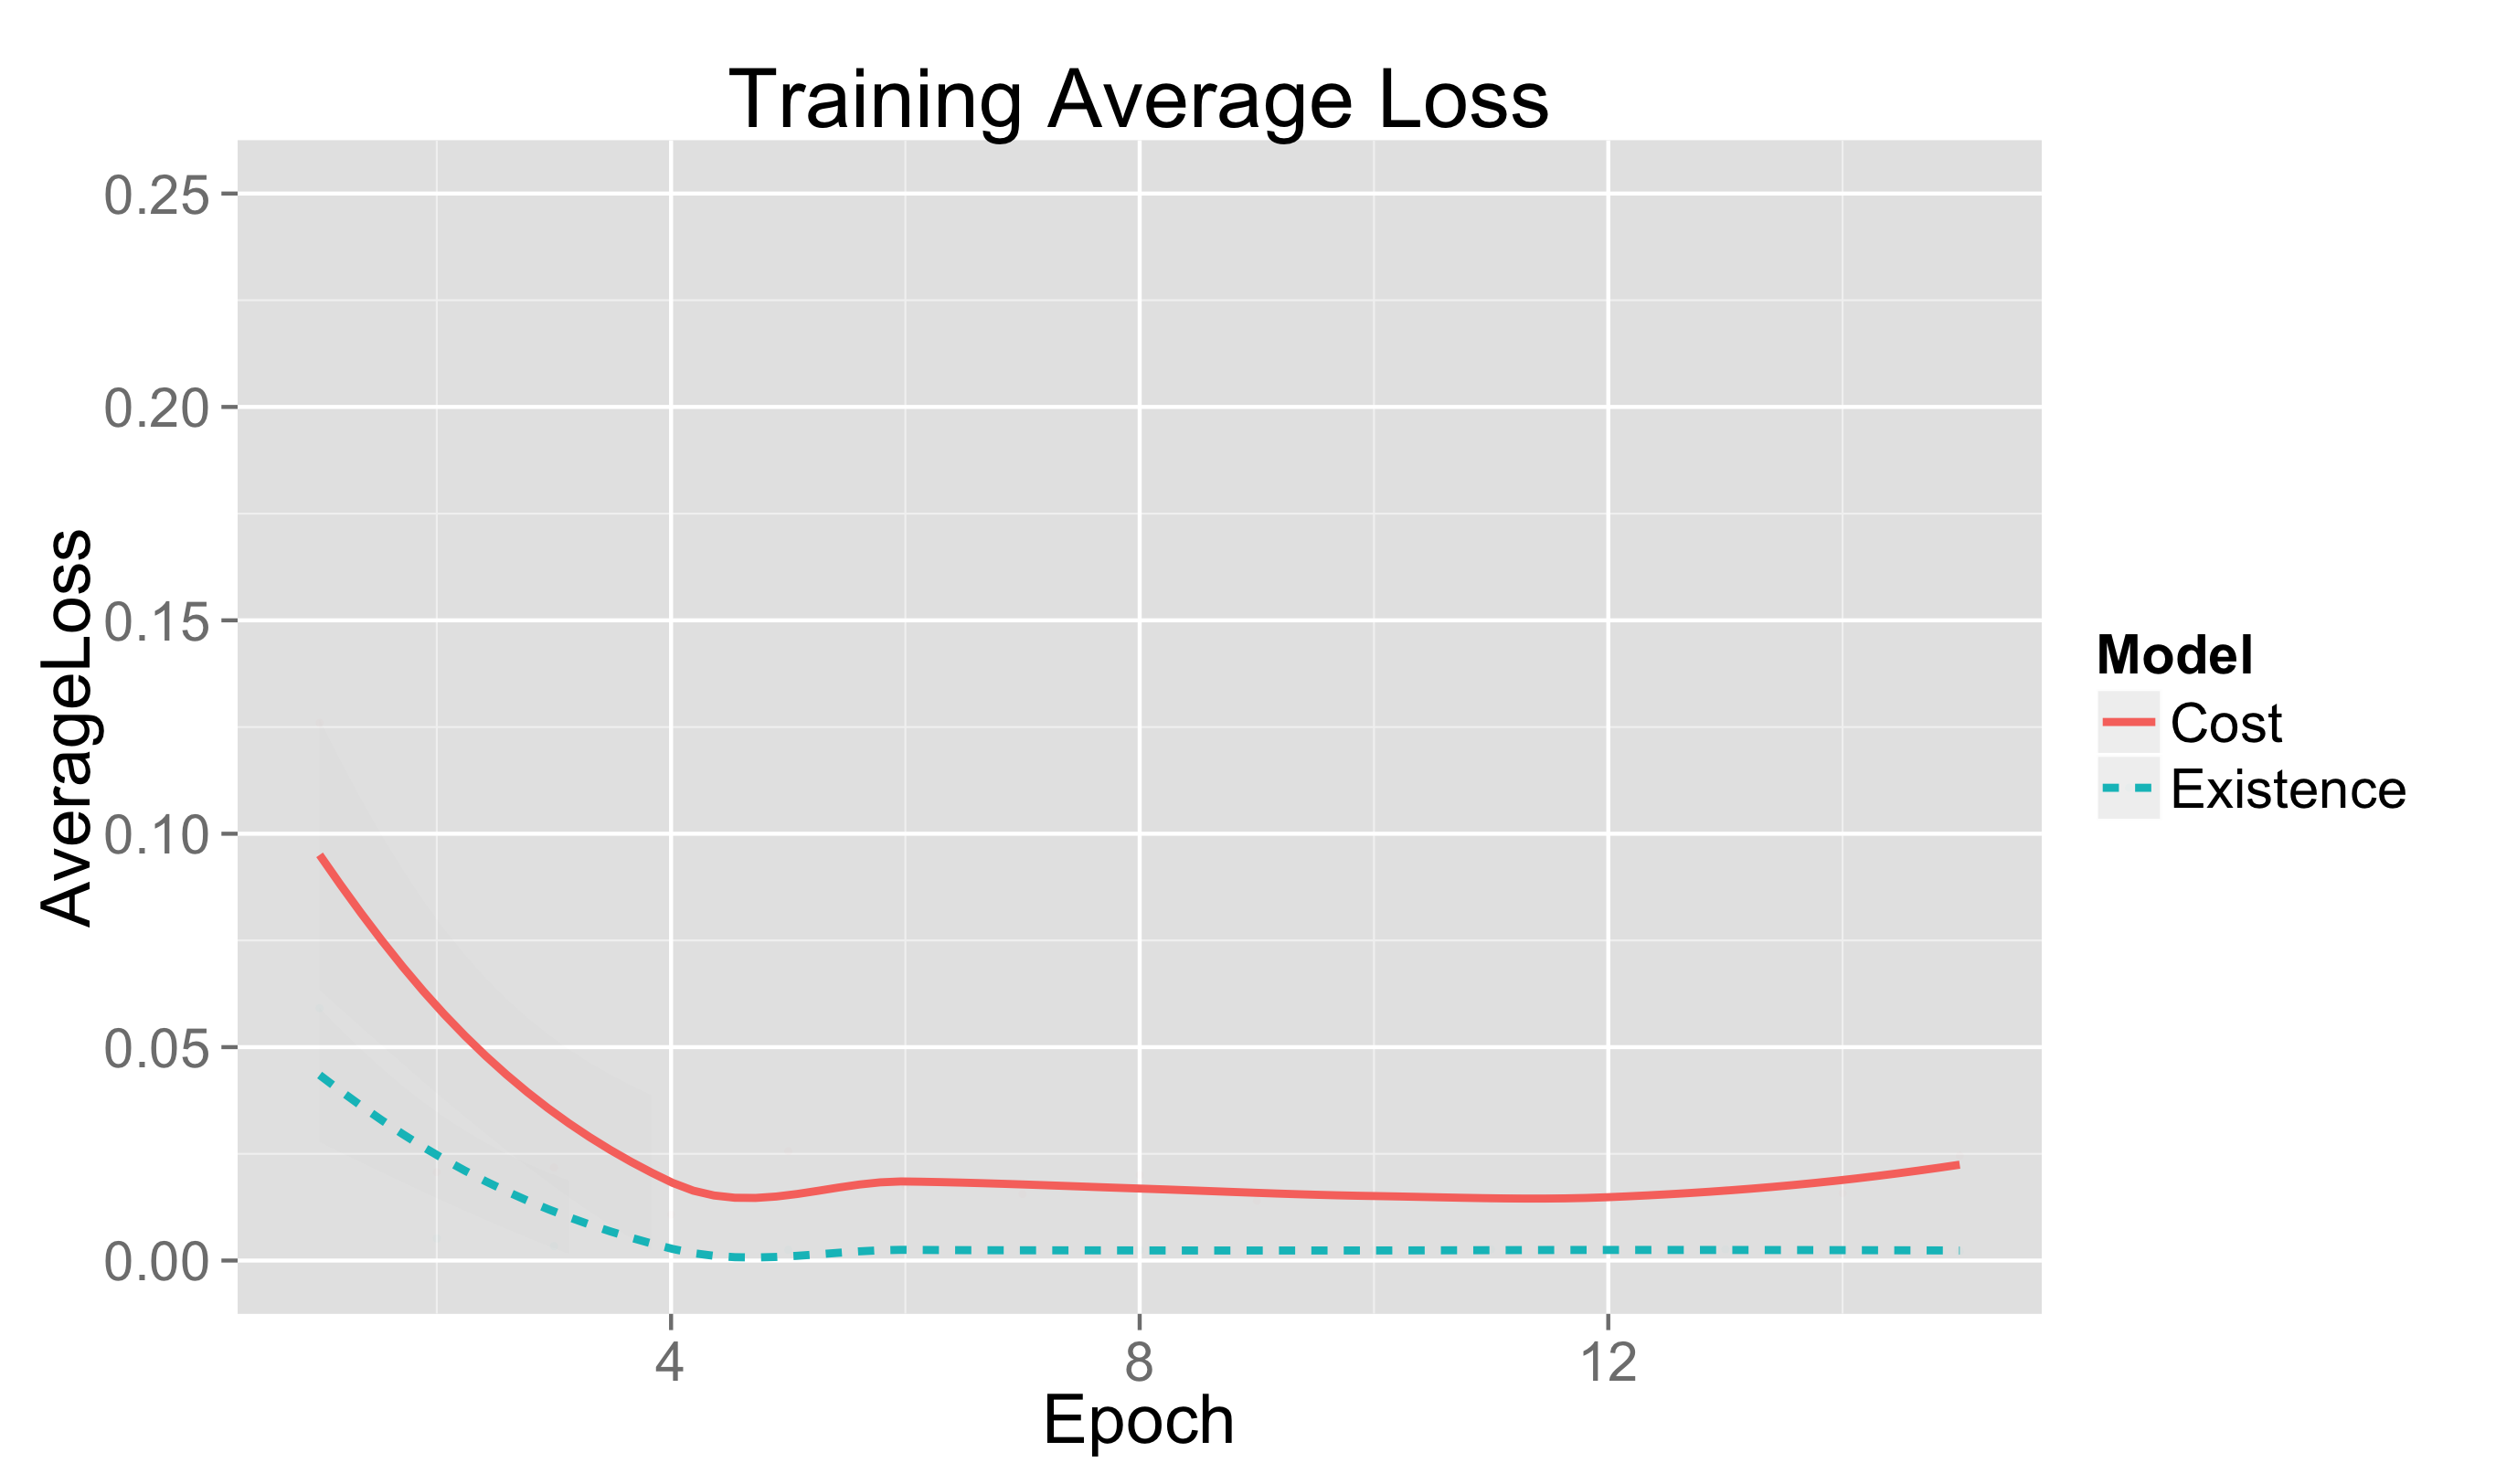
\includegraphics[scale=.1]{trainingAverageLoss.png}
  \end{center}
  \caption{Average training losses per epoch}
  \label{fig:avgloss}
\end{figure}

\subsection{Graph Prediction Performance}

As mentioned previously, the test graphs for epochs 16 through 20 are not
provided to contestants.  In order to determine the performance of graph
prediction, training data from epochs 1 through 10 \emph{only} were used to
train the model.  Then the graphs for epochs 11 through 15 were predicted
and compared against the training graphs for epochs 11 through 15.  The
results can be seen in Figure~\ref{fig:fscore}.  For both models performance
degrades over time, as anticipated, as the model has less history upon which
to form its prediction.  Note that the existence model degrades more rapidly
than the cost model.  The cost model has better performance for at least
three reasons (1) it was trained with both positive and negative data (2)we
only predict cost if we have already determined that the edge exists, and
(3) we observed in the training data that edges only change cost 2.6\% of
the time so the cost history backfilling strategy works well.

\begin{figure}
  \begin{center}
    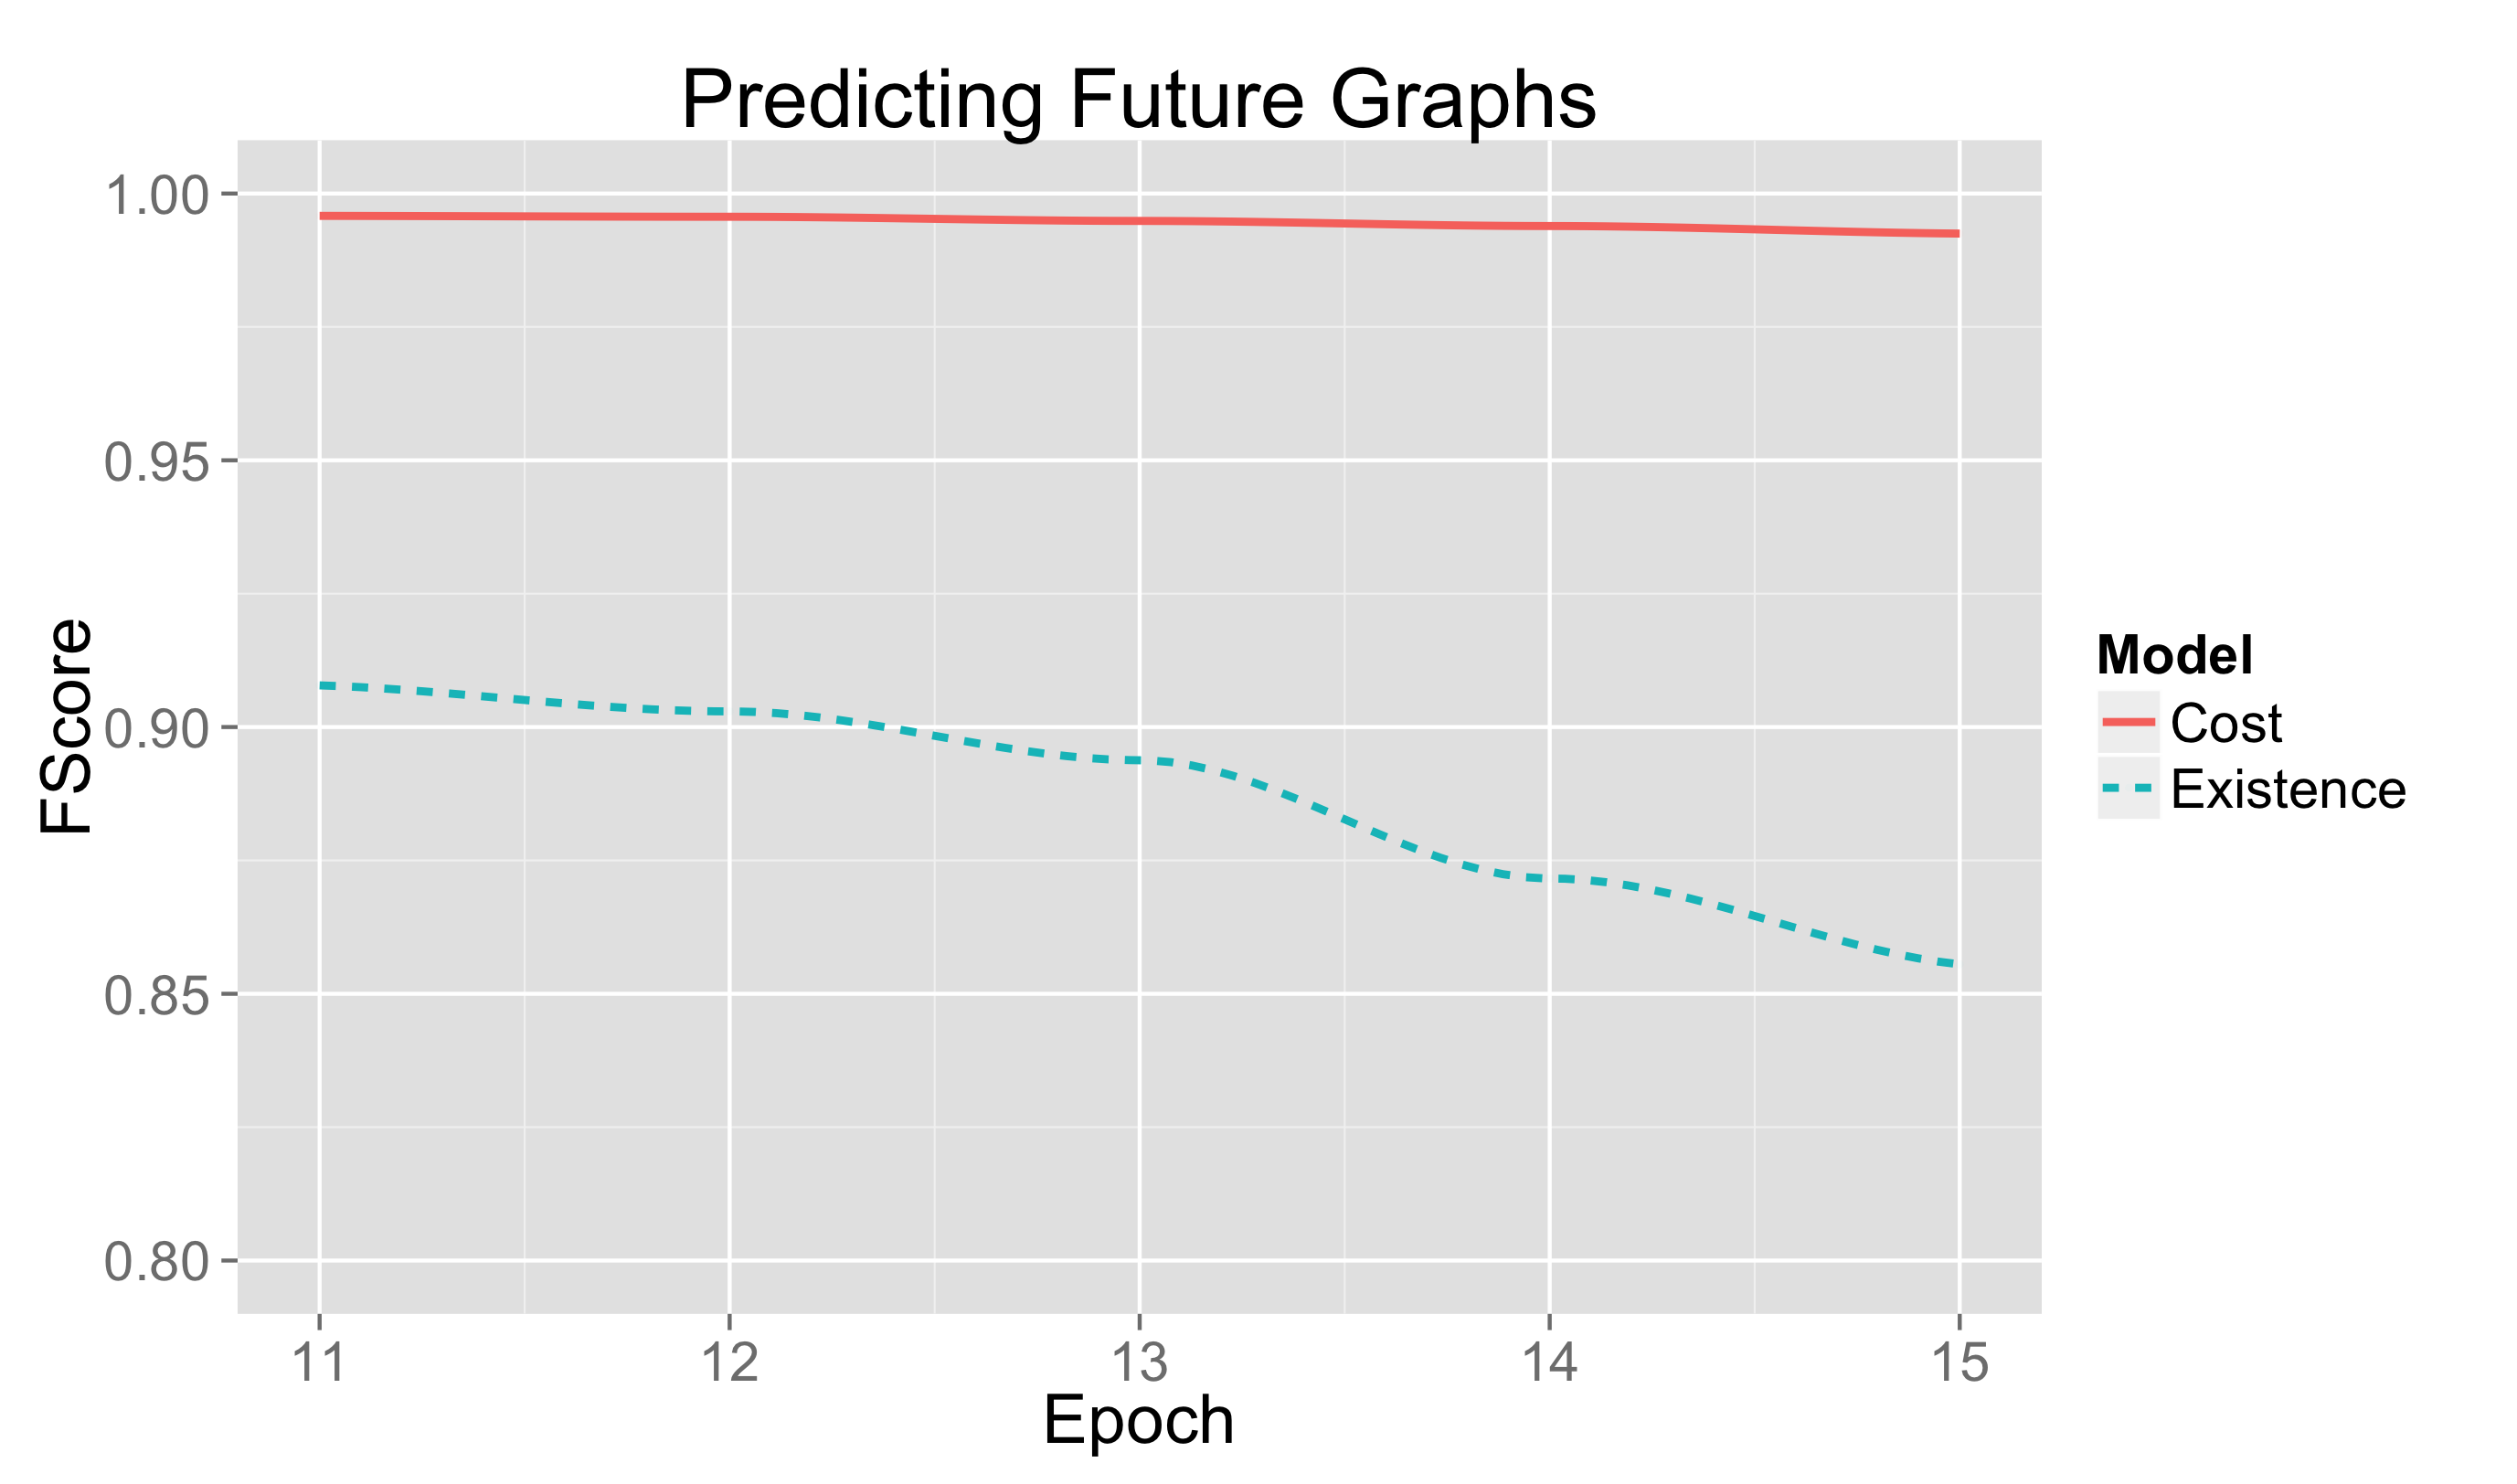
\includegraphics[scale=.1]{predictingFutureGraphs.png}
  \end{center}
  \caption{F-Score of predicted future graphs}
  \label{fig:fscore}
\end{figure}

\subsection{Optimality Prediction Performance}

In order to determine the performance of optimality prediction, I performed
the second step in Section~\ref{sec-pred} upon both the training graphs and
predicted graphs for epochs 11 through 15.  From Figure~\ref{fig:optloss}
you can see that the loss starts out in the range of 20\% which makes sense
given the fact that the effect of existence model performance is
multiplicative since we are predicting the optimality of multi-edge paths.

\begin{figure}
  \begin{center}
    \includegraphics[scale=.08]{predictionAverageLoss.png}
  \end{center}
  \caption{Average Loss of Optimality Prediction}
  \label{fig:optloss}
\end{figure}

\subsection{Kaggle Leaderboard Position}

Kaggle leaderboard rankings are determined as follows: ``Your predictions
will be evaluated by the Area Under the ROC Curve (AUC) metric.  While the
ground-truth is binary, real-valued submissions are allowed. ``~\cite{kaggle}
Figure~\ref{fig:chance} shows the leaderboard position of 110 for a random
chance prediction which serves as the baseline for this project.
Figure~\ref{fig:score} shows the leaderboard position of 47 for the
optimality predictions of the 10,000 test paths in epochs 16 though
20 using the models trained with data from epochs 1 through 15.

Note that the benchmark model submitted by the contest creators is at
leaderboard position 36 as shown in Figure~\ref{fig:bm}.  It is described as
``This benchmark takes the mode over the 15 training graphs. If the given
path is optimal in the graph, it receives a value of 1. If not, it gets a
0. The mode is then taken over all 15 values.''

Computing the historical mode over my own normalized training data results
in a leaderboard position of 60 per Figure~\ref{fig:hm}.  If my data
cleaning process had performed as well as the one used by the contest
creators, the leaderboard position should have been the same as the
benchmark.  Therefore this demonstrates that my data cleaning process
accounts for -0.08791 of the final ROC Curve metric.

\begin{figure}
  \begin{center}
    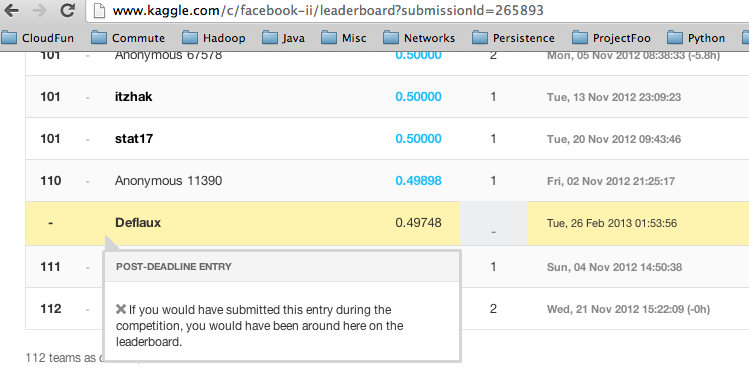
\includegraphics[scale=.4]{randomPredictions.png}
  \end{center}
  \caption{Random Chance Prediction Leaderboard Score}
  \label{fig:chance}
\end{figure}

\begin{figure}
  \begin{center}
    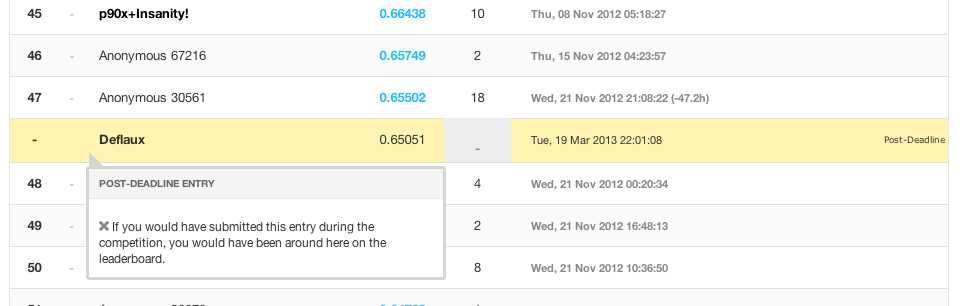
\includegraphics[scale=.4]{leaderboard.png}
  \end{center}
  \caption{Current Model Leaderboard Score}
  \label{fig:score}
\end{figure}

\begin{figure}
  \begin{center}
    \includegraphics[scale=.4]{benchmarkHistoricalModeLeaderboard.png}
  \end{center}
  \caption{Benchmark Historical Mode Leaderboard Score}
  \label{fig:bm}
\end{figure}

\begin{figure}
  \begin{center}
    \includegraphics[scale=.4]{historicalModeLeaderboard.png}
  \end{center}
  \caption{Historical Mode Leaderboard Score for predictions from normalized
    training graphs}
  \label{fig:hm}
\end{figure}

\pagebreak
\section{Next Steps}

Many different approaches could be taken to improve the performance of this model.

\begin{itemize}
\item improve the name cleaning process to bring the historical mode of my
  normalized training graphs closer to that of the benchmark model
\item fabricate negative existence data for training
\item penalize older history more heavily
\item try other ways to model recency of edges and also robustness
  of edges over time  (e.g., a recent edge may have come and go repeatedly so it
  should be considered ``flaky''; a specific example may be routers in India
  where the power situation is sporadic.)
\item use a min-count sketch~\cite{min} at each epoch to record the degree of each
node and use it in feature values for future time periods 
\end{itemize}

``For all of us sitting in front of our screens, the Internet only works
because every network is connected, somehow, to every other. So where do
those connections physically happen? More than most anywhere else, the
answer is `Ashburn.'''~\cite{tube}  

\small{
\begin{thebibliography}{99}

\bibitem{kaggle} \url{http://www.kaggle.com/c/facebook-ii/details/evaluation}

\bibitem{asn} \url{http://www.cisco.com/web/about/ac123/ac147/archived_issues/ipj_9-1/autonomous_system_numbers.html}

\bibitem{hash} Weinberger, Kilian, et al. {\it Feature hashing for large scale multitask learning." Proceedings of the 26th Annual International Conference on Machine Learning.} ACM, 2009.

\bibitem{rand} Nemirovski, Arkadi, et al. {\it Robust stochastic approximation approach to stochastic programming.} SIAM Journal on Optimization 19.4 (2009): 1574-1609.

\bibitem{online} Le Cun, Leon Bottou Yann. {\it Large Scale Online Learning.} Advances in
Neural Information Processing Systems 16: Proceedings of the 2003
Conference. Vol. 16. MIT Press, 2004.

\bibitem{min} Cormode, Graham, and S. Muthukrishnan. {\it An improved data
    stream summary: the count-min sketch and its applications.} Journal of
  Algorithms 55.1 (2005): 58-75.

\bibitem{tube} Blum, Andrew. {\it Tubes: A Journey to the Center of the
  Internet}. Ecco, 2012.

\end{thebibliography}
}

\end{document}
